\subsection{Support Model}
The support models are evaluated using several metrics, including macro F1 score, accuracy, balanced accuracy, and MCC.
The results are depicted in Figure \ref{fig:support_models_metrics}.\\
From the figure, it is evident that accuracy tends to be higher than other metrics for all models,
indicating a potential bias as it overestimates model performance.\\
Among the models, the MLP ensembles generally show superior performance compared to individual models.
Notably, the MLP\_Ensemble2 model exhibits the highest performance, with a macro F1 score of 81.58 and an MCC of 81.53.
This suggests that ensemble models effectively leverage the strengths of individual models to achieve optimal performance.
\begin{figure}[H]
    \centering
    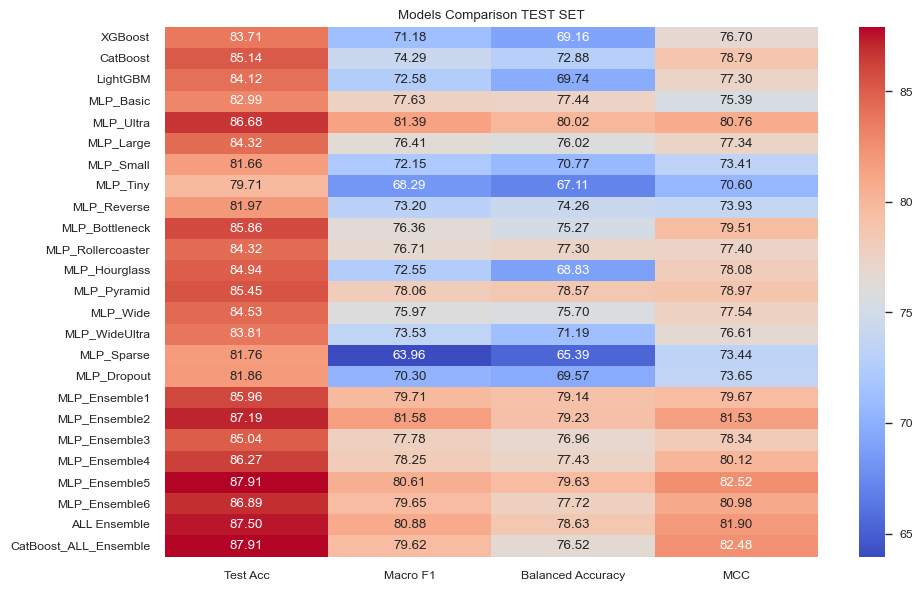
\includegraphics[width=1\columnwidth]{../images/support_models_metrics.png}
    \caption{Metrics of the Support Models, computed on the test set}
    \label{fig:support_models_metrics}
\end{figure}
\noindent
The risk of misclassifying an abnormal sample as normal is depicted in Figure \ref{fig:support_models_risk_scores},
 which shows the overall risk scores (in blue) for each model. The graph also displays specific risk scores associated with each class,
 representing the probability of predicting a sample of that class as normal.\\
This stacked bar chart helps compare the height of the different colors rather than their areas.
 From the figure, it's clear that no single model consistently outperforms others across all scores,but the performance varies across the scores. 
 For instance, MLP\_Rollercoaster has the best overall risk score (blue) and excels in murmurs risk score (red), 
 while MLP\_Ensemble3 performs best for extra systoles risk (orange).

\begin{figure*}[t]
    \centering
    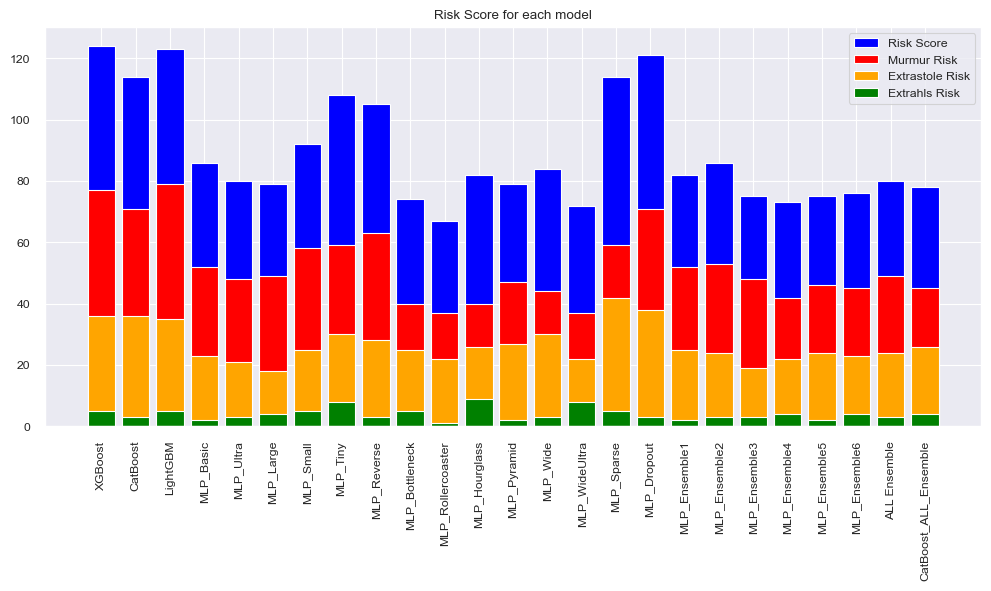
\includegraphics[width=0.8\textwidth]{../images/support_models_risk_scores.png}
    \caption{Risk Scores of the Support Models}
    \label{fig:support_models_risk_scores}
\end{figure*}

\subsubsection*{Best Model}

\begin{figure}[H]
    \centering
    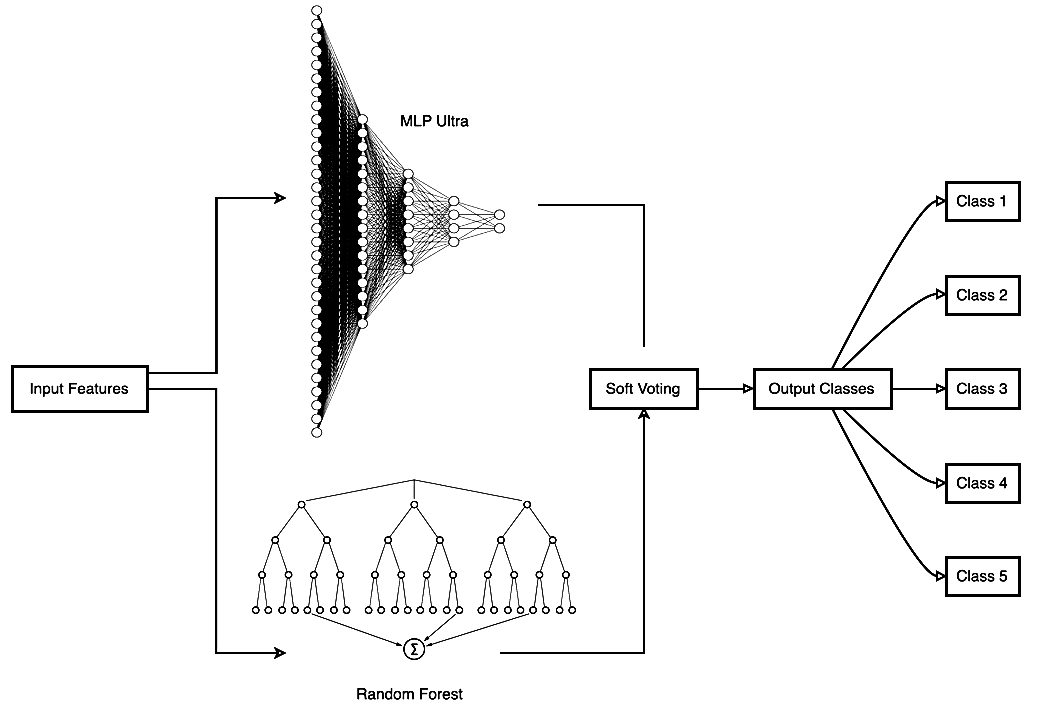
\includegraphics[width=0.8\columnwidth]{../images/MLP_Ensamble2.png}
    \caption{Architecture of the best Support Model}
    \label{fig:MLP_Ensamble2}
\end{figure}
\begin{figure}[H]
    \centering
    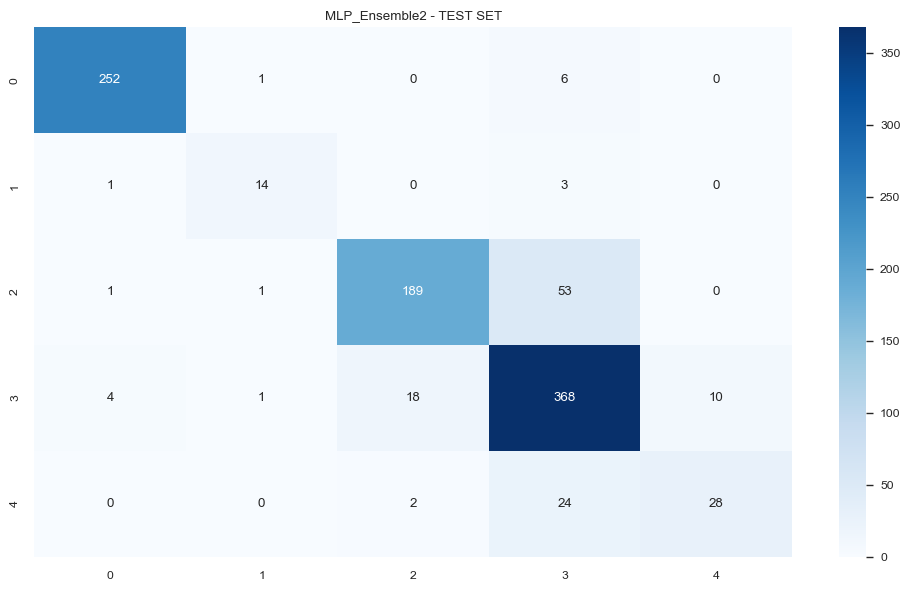
\includegraphics[width=0.8\columnwidth]{../images/support_models_conf_matrix.png}
    \caption{Confusion Matrix of the best Support Model}
    \label{fig:support_models_conf_matrix}
\end{figure}

\begin{figure*}[htpb]
    \centering
    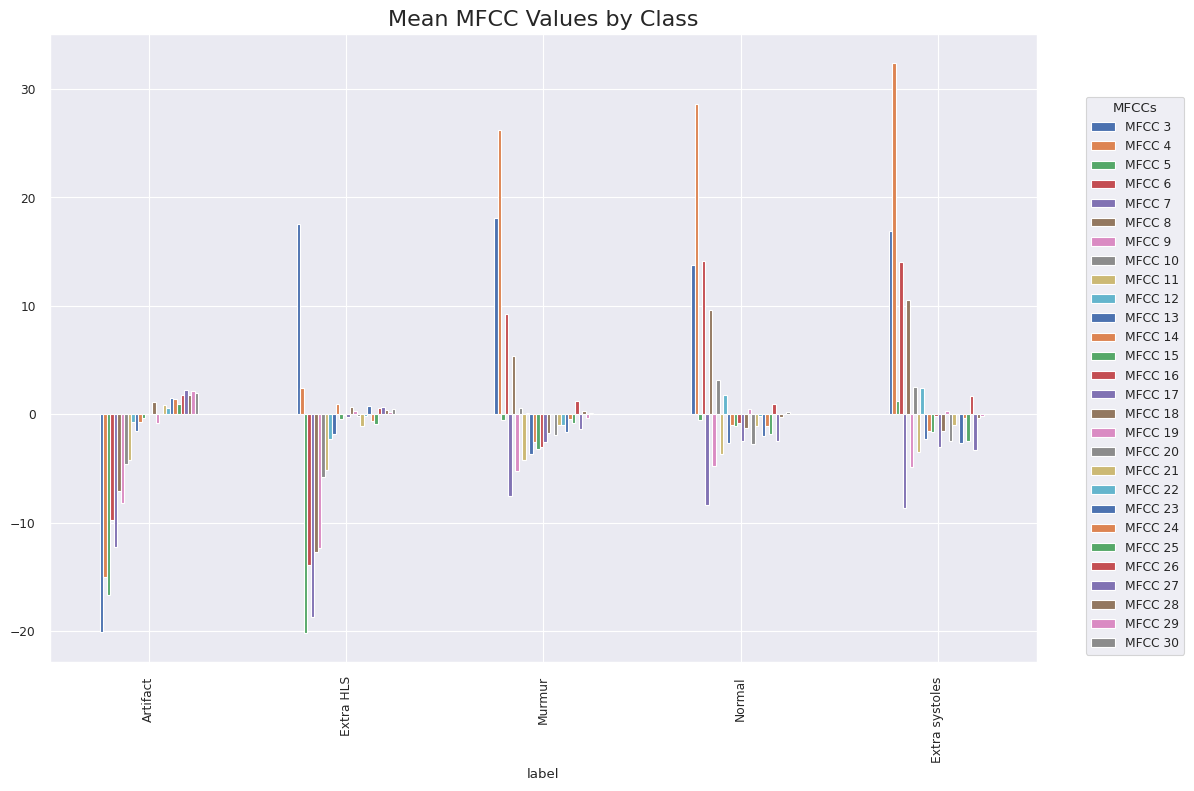
\includegraphics[width=0.8\textwidth]{../images/mean_val_for_features.png}
    \caption{Mean values for each feature within each class}
    \label{fig:mean_val_for_features}
\end{figure*}

\subsubsection*{Explainability}

\begin{figure*}[htpb]
    \centering
    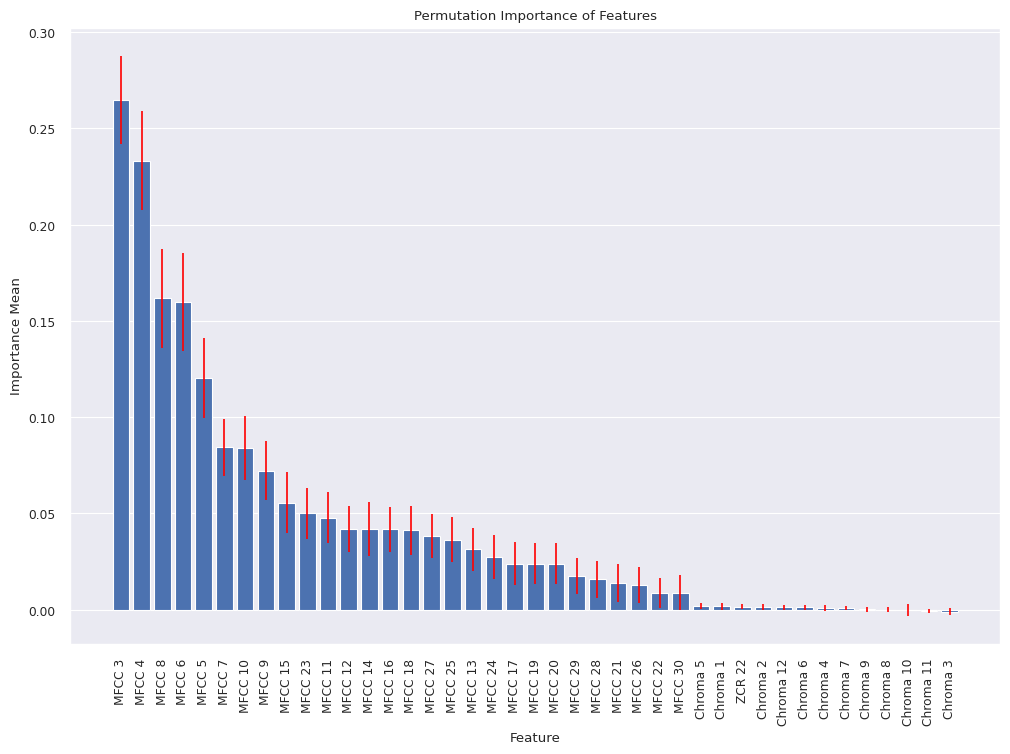
\includegraphics[width=0.8\textwidth]{../images/permutation_feature_importance.png}
    \caption{Feature Importance computed with Permutation Importance}
    \label{fig:permutation_feature_importance}
\end{figure*}


\begin{figure}[H]
    \centering
    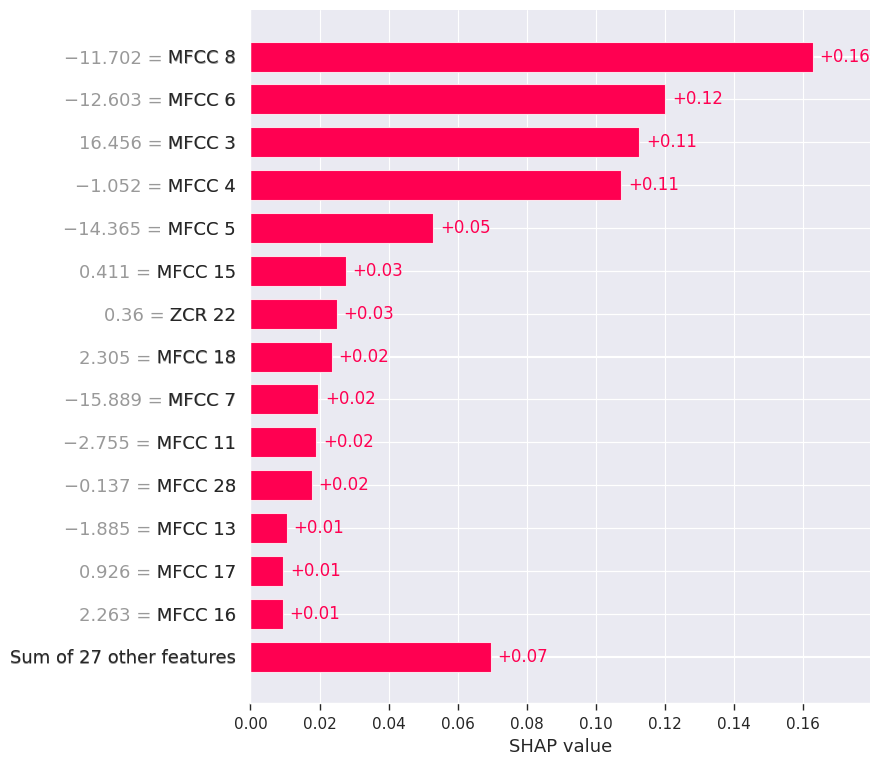
\includegraphics[width=0.8\columnwidth]{../images/extrahls_feature_importance.png}
    \caption{Feature importance for a single extra heart beat sample}
    \label{fig:extrahls_feature_importance}
\end{figure}